% !TEX encoding = UTF-8 Unicode
\documentclass[11pt, a4paper]{article}
\usepackage{authblk}
\linespread{1.2}
\usepackage{palatino}
\usepackage{parskip}
\usepackage{graphicx}
\usepackage[colorlinks,linktocpage]{hyperref}
\usepackage[listings]{tcolorbox}

% Title
\title{Manual for tsRFinder}
\author{Qinhu Wang}
\author{Weixing Shan\thanks{Email: wxshan@nwafu.edu.cn}}
\affil{Northwest A\&F University}
\date{Version 0.9\\[3pt] \today}

%%% Begin document
\begin{document}

\maketitle

\begin{abstract}
The tsRFinder is a lightweight, fast and reliable tool for transfer RNA-derived small RNA prediction and annotation with next-generating sequencing data. It's a free open source software available at: \url{https://github.com/wangqinhu/tsRFinder}.
\end{abstract}

\clearpage

\tableofcontents

\clearpage

\section{Introduction}

Small RNAs are key regulators of gene expression, such as miRNA, siRNA, and piRNA. The tRNA-derived small RNA (tsRNA; also called tRNA-derived RNA fragments, tRF), is a class of novel small RNA have been identified recently. However, there is no public tool specially tailored for tsRNA analysis yet. We thus developed tsRFinder for tsRNA prediction and annotation. It takes the small RNA sequencing data and the reference genome sequence, and identifies tsRNA with additional sequence and statistical analysis for you automatically.

\section{How to install}

\subsection{Dependencies}

The tsRFinder depends on a few free open source softwares, please check and install them \footnote{The dependencies version were based on the oldest environment we have tried.} at first:

\begin{itemize}

\item Perl, greater than v5.10.1, \underline{required}, for tsRFinder.pl execution.\\ Always build-in in most of the UNIX-like OS.
\item R, greater than v2.15.2, \underline{required}, for small RNA data analysis and illustration. \\\url{http://www.r-project.org}
\item bowtie, greater than v1.0.0, \underline{required}, for small RNA mapping. \\\url{https://github.com/BenLangmead/bowtie}
\item tRNAscan-SE, greater than v1.3.1, \underline{optional} if you want to prepare tRNA input yourself, for tRNA prediction. \\\url{http://lowelab.ucsc.edu/tRNAscan-SE}

\end{itemize}

\subsection{Installation}

tsRFinder is maintained on GitHub and is ready-to-use, no compilation is required. However, if you take some time to improve the configuration, it may save you a lot of time for trouble shooting.

First, you can clone \footnote{If git is not installed, download it from \url{http://git-scm.com}} tsRFinder by typing:

{\footnotesize \begin{tcolorbox}[colback=blue!5!white,colframe=blue!75!black,title=Clone tsRFinder]
\begin{verbatim}
git clone https://github.com/wangqinhu/tsRFinder.git
\end{verbatim}
\end{tcolorbox}}

in the terminal. Alternatively, you can download it from

{\footnotesize \begin{tcolorbox}[colback=blue!5!white,colframe=blue!75!black,title=Latest release of tsRFinder]
\begin{verbatim}
https://github.com/wangqinhu/tsRFinder/releases/latest
\end{verbatim}
\end{tcolorbox}}

and then decompress the zip file or the tarball.

When tsRFinder is cloned or unpacked, move the entire directory to a proper place (or current working directory, such as home directory) and add the tsRFinder path to your environment settings. For example, if tsRFinder is placed in /the/path/of/tsRFinder, then type the following in the terminal if you are using bash.


{\footnotesize \begin{tcolorbox}[colback=blue!5!white,colframe=blue!75!black,title=Setup tsRFinder]
\begin{verbatim}
echo export tsR_dir="/the/path/of/tsRFinder" >> ~/.bashrc
source ~/.bashrc
\end{verbatim}
\end{tcolorbox}}

And now, you can run tsRFinder for your dataset.

\section{How to use}

\subsection{Preparation the dataset}

Before running tsRFinder, you are asked to prepare/download the following two files: (1) the reference genome sequence, or the reference tRNA sequence and, (2) the small RNA reads.

We strongly recommend you using the reference genome sequence and the raw small RNA sequencing data, since tsRFinder can help you prepare the reference tRNA data and clean small RNA data automatically. If you want to prepare the tRNA file and small RNA reads file by yourself, you can run the demo data (enable debug mode in command line option: \emph{-m debug}) and find out which exact format of tRNA reference and small RNA reads file can be accepted instead, this is allowed but not encouraged. You can also found the format description in the FAQ part of this document.

\subsection{Running the pipeline}

tsRFinder supplies two ways for arguments input, you can use both configuration file and command line option. We recommend you using a command line option for debugging and building your configuration file. Once your inputs have been determined, you can write it to a configuration file for your analysis.

If tsRFinder is properly installed, you can run tsRFinder from your terminal directly, see the usage below.

{\footnotesize \begin{tcolorbox}[colback=blue!5!white,colframe=blue!75!black,title=Usage of tsRFinder: ./tsRFinder.pl -h]
\begin{verbatim}

tsRFinder usage:

    tsRFinder.pl <option>

    -c  Configuration file
    -l  Label
    -g  Reference genomic sequence
    -t  Reference tRNA sequence
    -s  Small RNA sequence
    -a  Adaptor sequence
    -n  Min read length            [defalut 18]
    -x  Max read length            [default 45]
    -f  Small RNA family threshold [default 72]
    -w  tRNA with/without label    [defualt no]
    -m  mode, run/debug            [defualt run]
    -h  Help
    -v  Version

Example:

    tsRFinder.pl -c demo/tsR.conf

\end{verbatim}
\end{tcolorbox}}

\section{Demo}

To have a quick but rough overview that how tsRFinder looks like, see the the animated gif demo in doc/demo.gif or online.

\subsection{Demo data}

\textbf{Demo refseq}: we used serval random sequences embedded with some real tRNAs as pseudo reference genome sequence. This small sequence data in FASTA format can be accessed in the file "tsRFinder/demo/genome.fa". In your analysis, if you have a reference genome, just replace it; if you don't have reference genome sequence, you can use the reference tRNA sequence instead. Figure \ref{refseq} shows what a refseq file looks like.

\begin{figure}[htbp]
\begin{center}
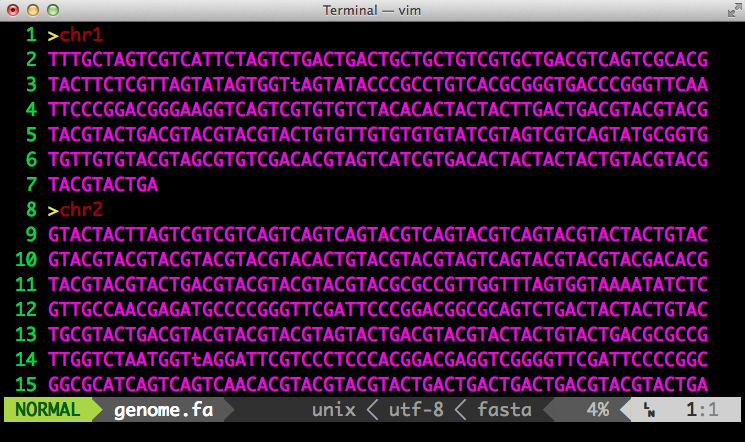
\includegraphics[width=12cm]{refseq.png}
\caption{Screenshot of the reference sequence in FASTA format} 
\label{refseq}
\end{center}
\end{figure}

\textbf{Demo sRNA}: we extracted a bit of raw reads from some real experimental data as a demo here. Each read of the raw small RNA data have 4 lines, just like what we have show in Figure \ref{fastq}.

\begin{figure}[htbp]
\begin{center}
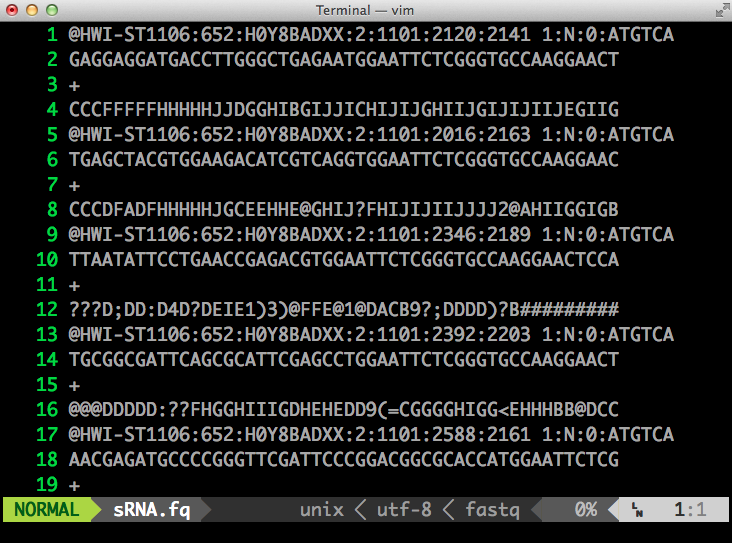
\includegraphics[width=12cm]{fastq.png}
\caption{Screenshot of the small RNA sequence in FASTQ format} 
\label{fastq}
\end{center}
\end{figure}

\subsection{Demo running}

tsRFinder allow you specify your inputs via a separate configuration file, for example, here is the content of our demo tsR.conf:

{\footnotesize \begin{tcolorbox}[colback=blue!5!white,colframe=blue!75!black,title=Demo configuration file for tsRFinder: demo/tsR.conf]
\begin{verbatim}
mode                :  run
label               :  Abc
reference_genome    :  demo/genome.fa 
reference_tRNA      :
sRNA                :  demo/sRNA.fq
adaptor             :  TGGAATTCTCGGGTGCCAAGG
min_read_length     :  18
max_read_length     :  45
family_threshold    :  72
tRNA_with_label     :  no
\end{verbatim}
\end{tcolorbox}}

Currently we have 10 items (13 options in command line) used for configuration file filling. The argument items and the inputs are separated by colon (":"). We recommend you using the first three letters of the organism you are analysing as a label (e.g. for \textit{Arabidopsis thaliana} we use \textit{Ath}, \emph{-l} in command line option); the paths of reference genome (\emph{-g}) and small RNA (\emph{-s}) should be supplied at least. If you are using a raw sequence data, please also input the adaptor sequence (\emph{-a}). If you are not using a reference tRNA (\emph{-t}) prepared by yourself, leave this argument to EMPTY please.

Once your configuration file is well prepared, typing the following in the terminal to run tsRFinder. In this demo, the configuration file (\emph{-c}) is at demo/tsR.conf, so we write like this:

{\footnotesize \begin{tcolorbox}[colback=blue!5!white,colframe=blue!75!black,title=Running tsRFinder demo]
\begin{verbatim}
./tsRFinder.pl -c demo/tsR.conf
\end{verbatim}
\end{tcolorbox}}

tsRFinder can work in run and debug modes (\emph{-m}), if you find some problem or want to extract some temporary files, you can enable debug mode, otherwise please use run mode (default). To check the usage or version, you can use \emph{-h} and \emph{-v} option, respectively.

\subsection{Demo output}

By default, tsRFinder will give you a summary of which files have been outputted and some basic statistics. The predicted or user inputed tRNA sequence, the small RNA clean data, the tRNA reads, and the predicted tsRNA sequence were listed. A figure showing the small RNA and tRNA reads length distribution (Figure \ref{distribution}) were included. Meanwhile, tsRFinder gives you additional summary on tsRNA family, tRNA/tsRNA expression (including 5' tsRNA and 3' tsRNA), text map (tmap) of small RNA mapped to tRNA, graphics showing the expression evaluated by small RNA data, the cleavage site, and also the cleavage profile (Figure \ref{cleavage}).
See our demo summary here:

{\footnotesize \begin{tcolorbox}[colback=blue!5!white,colframe=blue!75!black,title=tsRFinder demo output list]
\begin{verbatim}
---------
 SUMMARY 
---------

    tRNA seq : Abc/tRNA.fa
       Total : 5

  sRNA reads : Abc/sRNA.fa
       Total : 12472
      Unique : 7521

  tRNA reads : Abc/tRNA.read.fa
       Total : 283
      Unique : 50

   tsRNA seq : Abc/tsRNA.seq
       Total : 7
      Unique : 6

tsRNA report : Abc/tsRNA.report.xls

    text map : Abc/tsRNA.tmap

  visual map : Abc/images

distribution : Abc/distribution.pdf

    cleavage :
      detail : Abc/cleavage.txt
     profile : Abc/cleavage_profile.pdf

tsRNA family : Abc/tsRNA.fam

stat. by BDI :
 Sensitivity : 0.9593
 Specificity : 0.7825
    Accuracy : 0.8819

---------
\end{verbatim}
\end{tcolorbox}}

\begin{figure}[htbp]
\begin{center}
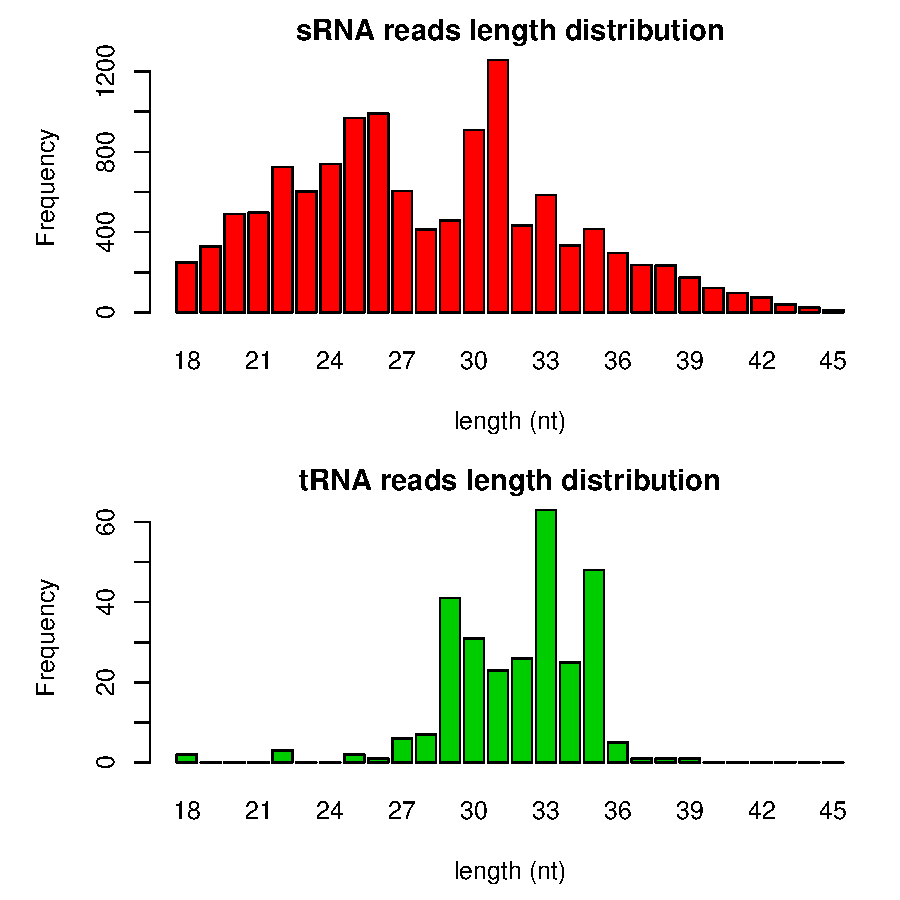
\includegraphics[width=13cm]{distribution.pdf}
\caption{Small RNA and tRNA reads distribution}
\label{distribution}
\end{center}
\end{figure}

\begin{figure}[htbp]
\begin{center}
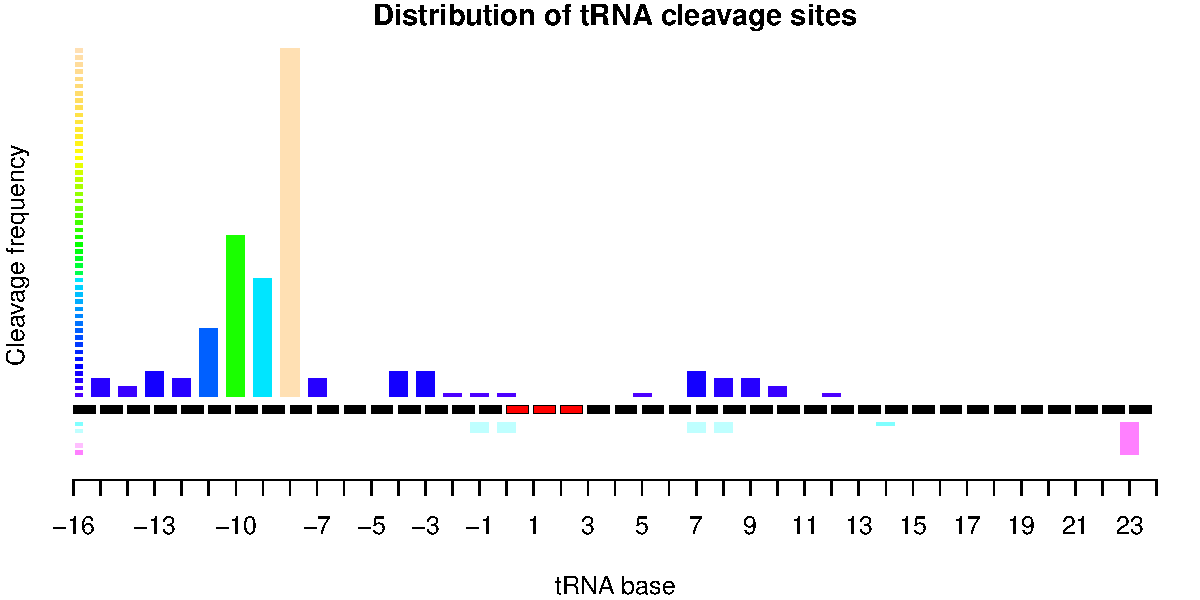
\includegraphics[width=13cm]{cleavage_profile.pdf}
\caption[Caption for LOF]{tRNA cleavage profile \footnote{This figure is based on public small RNA data GSM154336 and TAIR10, the demo data contains only a few reads and thus were not shown.}}
\label{cleavage}
\end{center}
\end{figure}

\subsection{Visualization of tmap data}

To examine the map of tsRNA, we developed a vim syntax plugin for visualization. If you want to enable color text map, copy lib/tmap.vim into your vim syntax folder, and put the following line into your .vimrc file:

{\footnotesize \begin{tcolorbox}[colback=blue!5!white,colframe=blue!75!black,title=Set filetype tmap in vim]
\begin{verbatim}
au BufNewFile,BufRead *.tmap  setf tmap
\end{verbatim}
\end{tcolorbox}}

When tmap.vim is correctly installed, open the tsRNA.tmap file with vim you will obtain a color text map, like Figure \ref{tmap}.

{\footnotesize \begin{tcolorbox}[colback=blue!5!white,colframe=blue!75!black,title=Visualization tsRNA.tmap]
\begin{verbatim}
vim tsRNA.tmap
\end{verbatim}
\end{tcolorbox}}

\begin{figure}[htbp]
\begin{center}
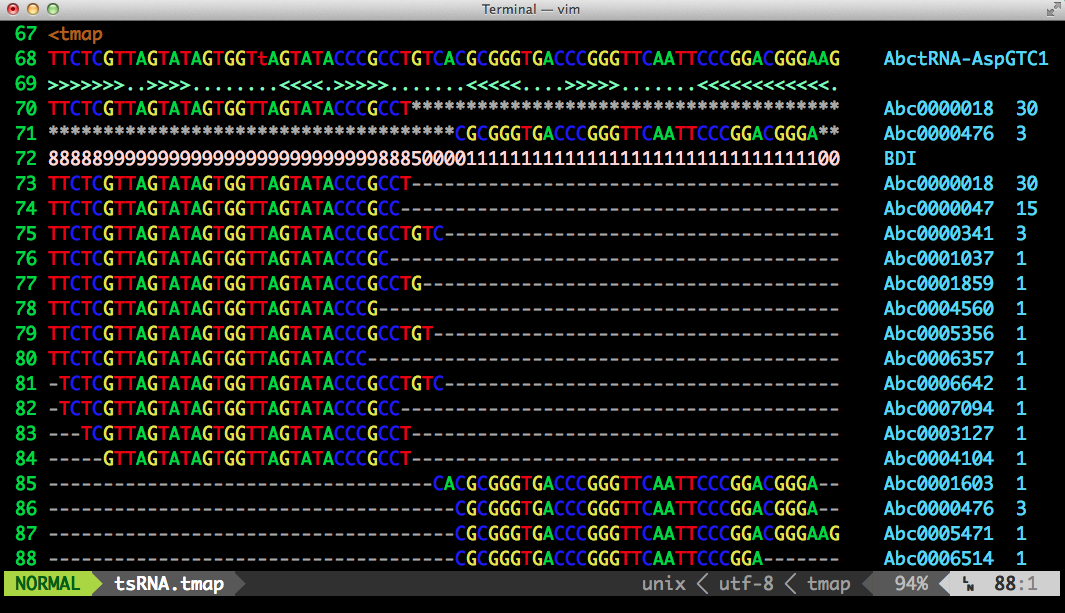
\includegraphics[width=12cm]{tmap.png}
\caption{Screenshot of color tmap} 
\label{tmap}
\end{center}
\end{figure}

If you prefer plain text view without highlighting, just open tsRNA.tmap with any kind of text editors you have.

\section{FAQ}

\textbf{1. Can tsRFinder run on Windows?}

No. tsRFinder depends on tRNAScan-SE (UNIX source code) and use some build-in program of UNIX-like systems, for example, awk, grep and head, thus running on Windows may lead unexpected errors, we strongly recommend you running tsRFinder on Linux or OS X.

\textbf{2. What's the length required for small RNA reads?}

Ideally, we recommend you sequencing from 15 - 50 nt for small RNA. However, 18 - 30 nt is OK if your tsRNA is shorter than 30 nt (such as tRF).

\textbf{3. What's the tRNA format required for input?}

At first we encourage you using a reference genomic sequence to instead it, since tsRFinder will help you extracting the tRNA sequence via tRNAscan-SE, removing duplicated sequences, and formatting input. And if you really want to use a file prepared yourself, please follow this format (see the example): first line, begin with "$>$", followed by label "$Abc$", then which tRNA "$tRNA-ProCGG1$";  second line, the sequence of the tRNA; and third line, the secondary structure of tRNA, "$><$" and "$()$" both were acceptable. But becareful because ">" equals "(" but not ")". 

{\tiny \begin{tcolorbox}[colback=blue!5!white,colframe=blue!75!black,title=tRNA example]
\begin{verbatim}
>AbctRNA-ProCGG1
GGCCTCGTGGTCTAGTGGTATGATTCTCGCTTCGGGTGCGAGAGGtCCCGGGTTCGATTCCCGGTGAGGCCC
>>>>>>>..>>>.........<<<.>>>>>.......<<<<<.....>>>>>.......<<<<<<<<<<<<.
\end{verbatim}
\end{tcolorbox}}

\textbf{4. What's the sRNA format required for input?}

We recommend you using a raw data. To have an sRNA file for input prepared yourself, please follow this format (see example): first line, begin with "$>$", then the label "$Abc$", then the 7\-bit index, followed by "$\_$" (or "$|$", "$-$" and white space) and the read number; second line, the sequence of the read. One more thing, tsRFinder sRNA data format is compatible with FASTX\_TOOL kit \footnote{\url{http://hannonlab.cshl.edu/fastx_toolkit/}}, so you can prepare this with fastx tools. 

{\tiny \begin{tcolorbox}[colback=blue!5!white,colframe=blue!75!black,title=sRNA example]
\begin{verbatim}
>Abc0000001_772
CAGGTGGTCAGGTAGAGAATACCAAGGCGCT
>Abc0000002_475
AGGTGGTCAGGTAGAGAATACCAAGGCGCT
\end{verbatim}
\end{tcolorbox}}


\textbf{5. I have problem in installing tsRFinder and/or the dependencies, where to get more help?}

You can go to the official support website or create new issue for tsRFinder repository on GitHub. The URL is \url{https://github.com/wangqinhu/tsRFinder/issues/new}

\textbf{6. Where to report bugs?}

Goto \url{https://github.com/wangqinhu/tsRFinder/issues/new}

\textbf{7. Can we use tsRFinder for commercial purpose?}

Yes. tsRFinder is free, open source software, see the MIT license.

\textbf{8. The 'nwalign' is not suit for my operating system, what can I do?}
 
tsRFinder using Needleman-Wunsch algorithm nwalign for small RNA alignment, we pre-build the binaries for some of the recently OS X / Linux, if you find it not suitable for your system or want to compile it by your self, goto lib/src directory and type 'make' to build \footnote{The gcc compiler is required. For OS X, you can install Xcode (ship with gcc)} it.

\end{document}
